% Comando simples para exibir comandos Latex no texto
\newcommand{\comando}[1]{\textbf{$\backslash$#1}}

\section{Documentos Fiscais Eletrônicos}
\label{introducao:dfe}

Segundo dados da \citeonline{receita:dados-publicos:cnpj}, o Brasil possuía em setembro de 2020 mais de 45 milhões de empresas ativas que realizam transações todos os dias envolvendo aquisição e transferência de mercadorias, prestação de serviços das mais diversas naturezas, transportes e devoluções. Essas empresas possuem uma série de obrigações contábeis e fiscais a cumprir todos os meses. Obrigações essas que se traduzem em documentos enviados ao governo contendo uma série de informações sobre cada uma dessas transações efetuadas.

A lei que obriga a emissão de notas fiscais é datada do ano de 1994~\cite{lei:8846:documentos-fiscais}. À época, a emissão desses documentos era feita em papel, o que causava grandes transtornos às empresas tanto por conta dos próprios processos envolvidos quanto por conta da guarda desses documentos, que a depender do porte e do volume de transações das empresas exigia um grande esforço de armazenamento de milhares de documentos todos os meses. Era comum nas empresas a presença arquivos de aço para a guarda desses documentos.

A modernização da legislação que aconteceu na década seguinte possibilitou a diminuição desse problema, e através de parcerias entre os governos foi possível informatizar esses processos e o que era então papel passou a ser arquivo eletrônico armazenado em computadores ou servidores, viabilizando também a automação desses processos. Esse processo de modernização, ocorrido também em vários países da América Latina, é descrito por \citeonline{mello2014documentos} que relata uma convergência entre vários países para o uso de tecnologias semelhantes, como a estruturação dos dados em arquivos XML, a existência de uma versão impressa, como o \sigla{DANFE}{Documento Auxiliar da Nota Fiscal Eletrônica} e o \sigla{DACTE}{Documento Auxiliar do Conhecimento de Transporte Eletrônico}, o uso de assinaturas digitais para verificação de autenticidade e autoria, e o uso de \textit{web services} para a emissão e disponibilização desses documentos. \citeonline{pasa2001uso} descreve uma série de normas e recomendações que viabilizam o uso de documentos fiscais de forma confiável e legalmente viável e fala da necessidade de "transformar o contador em um verdadeiro analista de informação".

Outro importante ganho advindo da informatização desses documentos foi justamente a facilitação do uso desses documentos para não só cumprir obrigações contábeis e fiscais, mas também em processos internos de empresas e até mesmo análises financeiras e econômicas de diversas finalidades. Os \sigla*{DFe}{Documento Fiscal Eletrônico} documentos fiscais eletrônicos são ricos em informações, contendo dados detalhados de forma estruturada acerca das transações efetuadas entre empresas, onde são descritos produtos, valores, impostos, e classificações que possuem uma infinidade de aplicações.

Alguns trabalhos acadêmicos já exploraram anteriormente algumas dessas aplicações através do uso de documentos fiscais para propor soluções para a sociedade. \citeonline{fernandez2012avaliaccao} propõe o uso de documentos fiscais, como a \sigla{NFe}{Nota Fiscal Eletrônica}, o \sigla{CTe}{Conhecimento de Transporte Eletrônico}, e do \sigla{MDFe}{Manifesto Econômico de Documentos Fiscais} para o rastreamento de cargas e veículos, os tornando importante ferramentas de prevenção e combate à sonegação e fraudes. O trabalho de \citeonline{madeira2015aplicaccao} também propõe um método de mineração de texto para a detecção de fraudes e incorreções através de dados de Notas Fiscais de Serviços Eletrônicas, classificando-as quanto a essas incorreções com métodos computacionais.

Outra aplicação é apresentada no trabalho de \citeonline{santos2015uso}, que aplica o uso de dados de NFes no estudo de alternativas para a obtenção de dados para o planejamento do transporte de cargas urbano, como forma de levantar dados para a tomada de decisões que evitem congestionamentos ou otimizem fluxos de tráfego devido a esse tipo de transporte.

Por fim, o trabalho de \citeonline{campos2019geraccao} faz o uso de MDFes para a obtenção de matrizes Origem-Destino, uma ferramenta de visualização de demanda, mostrando em seus resultados que as matrizes obtidas através de dados de documento fiscais eram semelhantes às obtidas com métodos tradicionais.

Todos esses trabalhos atestam a riqueza, viabilidade, e confiabilidade dos dados de documentos fiscais para uso em variados domínios e aplicações.

\section{A Pandemia de COVID-19}
\label{introducao:pandemia}

O ano de 2020 foi marcado por uma pandemia de proporções globais poucas vezes vista na história da humanidade. Segundo \citeonline{zhou2020pneumonia}, a epidemia se iniciou no dia 12 de dezembro de 2019 na cidade de Wuhan, na China, causada por infecções pelo coronavírus Sars-Cov-2 capaz de causar Síndrome Respiratório Aguda Grave, doença chamada COVID-19, cujos sintomas incluem febre, tosse seca, dificuldade respiratória, dor de cabeça, podendo evoluir para casos mais graves com pneumonia, danos pulmonares, e morte.

Em 26 de fevereiro de 2020, o Brasil confirmou seu primeiro caso de infecção pelo vírus em um paciente de 61 anos vindo da Itália \cite{artigo:folha:primeiro-caso}, e sua primeira morte no dia 17 de março de 2020 na cidade de São Paulo, um homem de 62 anos \cite{artigo:folha:primeira-morte}. O preocupante espalhamento do vírus por diversos países levou a Organização Mundial da Saúde a declarar em 11 de março de 2020 à classificação de pandemia \cite{artigo:folha:oms-declara-pandemia}, após a disseminação para mais de cem países em todos os continentes.

A OMS recomenda como forma de prevenção o distanciamento social, o uso de máscaras, e a higiene contínua das mãos \cite{oms:coronavirus-disease-advice}. O alto risco de contaminação por pacientes assintomáticos e pressintomáticos infectados torna o controle da doença muito difícil, sendo os principais métodos populacionais de prevenção indicados o isolamento e a quarentena \cite{oms:coronavirus-faq}. A doença ainda não possui remédios eficazes indicados pela OMS, sendo recomendados apenas a prevenção e tratamentos intensivos para pacientes já em estado grave.

O Brasil, assim como diversos países do mundo, adotou medidas para conter o avanço do vírus. Por meio da lei nº 13.979/2020 \cite{lei:13979:medidas-para-pandemia}, alterada posteriormente pelas leis nº 14.019/2020 \cite{lei:14019:medidas-para-pandemia} e 14.035/2020 \cite{lei:14035:medidas-para-pandemia}, foram estabelecidas medidas para enfrentamento da pandemia, que no Artigo 3º prevê:

\begin{citacao}
Art. 3º  Para enfrentamento da emergência de saúde pública de importância internacional de que trata esta Lei, as autoridades poderão adotar, no âmbito de suas competências, entre outras, as seguintes medidas:

I - isolamento;

II - quarentena;

III - determinação de realização compulsória de:

a) exames médicos;
    
b) testes laboratoriais;
    
c) coleta de amostras clínicas;
    
d) vacinação e outras medidas profiláticas; ou 
    
e) tratamentos médicos específicos;
    
III-A – uso obrigatório de máscaras de proteção individual; 

...

VI – restrição excepcional e temporária, por rodovias, portos ou aeroportos, de: 

a) entrada e saída do País; e
    
b) locomoção interestadual e intermunicipal;
\end{citacao}

A adoção dessas medidas, embora não tem ocorrido de forma ordenada em todo o país, afetou a mobilidade social. Como exemplo de tais medidas, no dia 21 de março de 2020 o governo do estado de São Paulo \cite{artigo:folha:sp-fechamento-comercio} decreta o fechamento do comércio e de todos os serviços essenciais por 15 dias, medida posteriormente prolongada cujos efeitos duraram várias semanas. Também na cidade do Rio de Janeiro, foi decretado o fechamento obrigatório do comércio no dia 22 de março de 2020, também em tentativa de conter o vírus \cite{artigo:uol:rj-fechamento-comercio}. No dia 18 de maio de 2020, a cidade de São Paulo aprovou a antecipação de dois feriados \cite{artigo:folha:sao-paulo-aprova-feriados} como forma de incentivar o aumento do índice de isolamento social, que indica o percentual da população que está efetivamente respeitando o isolamento social.

A Figura~\ref{fig:intro-1.1-isolamento-social-brasil} ilustra como o índice de isolamento social variou entre fevereiro de 2020 e janeiro de 2021. O pico de isolamento ocorreu no dia 22 de março de 2020 alcançando 62.2\%, mas posteriormente diminuiu estando no patamar de 37.3\% em 15 de janeiro de 2021.

\begin{figure}[htb]
    \centering
    \caption{Gráfico do índice de isolamento social no Brasil}
    \label{fig:intro-1.1-isolamento-social-brasil}
    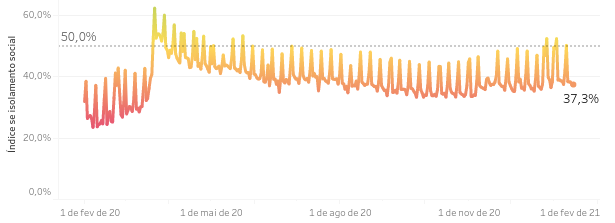
\includegraphics[scale=0.7]{images/intro-1.1-isolamento-social-brasil.png}
    \fdireta{inloco:mapa-isolamento-brasil}
\end{figure}

Em janeiro de 2021, a OMS registra mais de 90 milhões de casos confirmados de infecção, sendo mais de 2 milhões de mortes causadas pela doença \cite{oms:coronavirus-disease-dashboard}, sendo que a cada dia estão ainda sendo registrados em média cerca de 100 mil novos casos e 2 mil mortes. O Brasil registra mais de 8 milhões de casos confirmados sendo 200 mil mortes causadas pela doença, sendo ainda registrados em média cerca de 50 mil casos e 1 mil mortos por dia. No momento, a OMS avalia 15 vacinas candidatas a imunizantes, algumas já com pesquisas avançadas e em uso emergencial por alguns países \cite{oms:coronavirus-vaccines-status}.

O Brasil aplicou seu primeiro imunizante \cite{artigo:folha:primeira-vacina} no dia 17 de janeiro de 2021, após aprovação para uso em caráter emergencial pela \sigla{Anvisa}{Agência Nacional de Vigilância Sanitária}, em uma enfermeira de 54 anos que trabalha na UTI do Instituto de Infectologia Emílio Ribas, em São Paulo.

\section{Crise econômica}
\label{introducao:crise-economica}

O fechamento do comércio, as medidas de incentivo ao isolamento social, além dos altos números de mortos, são fatores que afetam economicamente diversos setores da economia.

\citeonline[traduç{\~a}o nossa]{mckibbin2020economic} aponta que "em um mundo fortemente conectado e integrado, os impactos da doença (COVID-19) vão além da mortalidade (aqueles que morrem) e da morbidade (aqueles que ficam incapazes de trabalhar por um período de tempo)". O estudo, datado de março de 2020, ainda previa cenários onde a pandemia poderia se manter restrita à China, mas também a cenários que hoje sabemos mais próximos da realidade com a doença se espalhando por diversos países. Este estudo já apontava a possibilidade, hoje confirmada, de um alto número de mortes e alto impacto no \sigla{PIB}{Produto Interno Bruto} nos países estudados. Mesmo nos cenários mais otimistas, de menor espalhamento do vírus, o estudo já previa um desvio negativo importante para o PIB de diversos países, podendo chegar a 9.9\% de desvio negativo nos piores casos. Segundo os dados do \sigla{IBGE}{Instituto Brasil de Geografica e Estatística}, o Brasil teve no acumulado entre o último trimestre de 2019 e os três primeiros trimestres de 2020 uma queda de 3.4\% no PIB \citeonline{intro:ibge-pib}.

O trabalho de \citeonline[traduç{\~a}o nossa]{fernandes2020economic} faz uma análise dos impactos econômicos da COVID-19 no cenário mundial ainda em março de 2020. O estudo aponta que "os impactos da doença vão além da mortalidade. Sendo que, governos por todo mundo tem se preparado para planos de contingência e pacotes de ajuda para sustentar suas economias', apontando também para o impacto dos \textit{lockdowns}, uma das medidas restritivas adotadas, na redução do consumo e em interrupções na produção. O estudo também compara o evento de 2020 com crises anteriores e descreve que tanto em relação à crise econômica de 2008 quanto em relação à pandemia de SARS de 2002 há diferenças signiticativas que tornam a crise de 2020 mais grave e abrangente.

Em outro estudo, \citeonline{sun2020did} analisa o impacto da pandemia no transporte aéreo global e como este poderia ter contribuído para a pandemia, usando dados de radares aéreos do mundo todo. Neste trabalho, \citeonline{sun2020did} mostra uma diminuição da conectividade em um grafo de conexões em aeroportos de todo o mundo se comparado o mês de janeiro com o mês de maio de 2020. Ao comparar métricas de sistemas complexos neste período, o estudo também detecta uma queda de 50\% na centralidade de grau, uma redução também da assortatividade de grau, um aumento significativo na centralidade de intermediação, e também na quantidade de comunidades da rede. Este estudo é um precedente importante para o nosso trabalho uma vez que aponta a alterações topológicas em sistemas complexos causadas pela pandemia.

Usando dados do mercado de ações, \citeonline{aslam2020network} faz uma análise da variação da correlação entre diversos mercado e mudanças estruturais do ponto de vista de sistemas complexos entre o período anterior e durante o espalhamento da COVID-19. Este estudo também identifica mudanças topológicas no relacionamento entre mercado de todo o mundo, relatando um aumento do caminho mínimo médio entre eles, além de uma diminuição na centralidade de intermediação e na centralidade de proximidade. Essa análise considera apenas a árvore geradora mínima, mas já aponta mudanças diferentes das relatadas por \citeonline{sun2020did}.

Estudos sobre o impacto econômico da crise causada pela COVID-19 ainda serão complementados por outros trabalhos, tendo em vista que ainda não alcançamos e o fim da pandemia é difícil prever quando isso acontecerá, e também por ser um evento relativamente recente e que certamente ainda será muito analisado.

\section{Objetivos}
\label{introducao:objetivos}

Tendo em vista a oportunidade de utilizar valiosos dados de documentos fiscais, o impacto econômico previsto por outros trabalhos, e a importância do evento ocorrido, este trabalho se propõe a contribuir com uma análise do impacto econômico da crise provocada pela pandemia de COVID-19 através do ponto de vista de sistemas complexos, e com uma análise do impacto de mudanças topológicas de redes na magnitude e abrangência da crise para cada entidade estudada, apresentando uma categorização de impacto econômico, e verificando se há possibilidade de utilizar esses dados para categorizá-las entre entidades afetadas e não-afetadas pela crise.

No capítulo~\ref{chapter:documenos-fiscais} será apresentado o domínio dos dados utilizados neste trabalho com uma explicação sobre documentos fiscais, a legislação brasileira envolvida, e os sistemas usados para captação dos dados. A seguir, será descrita a base de dados utilizada, com uma análise descritiva e detalhes do pré-processamento feito para a coleta dos dados no capítulo~\ref{chapter:base-de-dados}. O impacto econômico da crise é descrito no capítulo~\ref{chapter:impacto-economico} que mostra sob diferentes visões a abrangência e magnitude da mesma. No capítulo~\ref{chapter:resultados} é feita uma análise descritiva com diferentes modelagens e métricas das redes utilizadas e são mostradas possíveis alterações estruturais no ponto de vista de sistemas complexos, com diferentes modelagens, e uma tentativa de identificação de características que podem levar a categorizar um agente econômico como afetado ou não pela pandemia. O capítulo~\ref{chapter:conclusão} encerra este trabalho com as conclusões obtidas e os próximos passos propostos por este trabalho.
